% Guía rápida de IPTV, edición en español. Compilar en esta carpeta con:
%   pdflatex IPTV-Quick-Start-es.tex   (dos veces, para el índice)
\newcommand{\GuideLang}{spanish}
\newcommand{\GuideTitle}{Guía rápida}
\newcommand{\TipLabel}{Consejo.}
% Shared layout of the IPTV quick start guides (one file per language:
% IPTV-Quick-Start.tex, IPTV-Quick-Start-it.tex, ...). Each sets, before
% % Shared layout of the IPTV quick start guides (one file per language:
% IPTV-Quick-Start.tex, IPTV-Quick-Start-it.tex, ...). Each sets, before
% % Shared layout of the IPTV quick start guides (one file per language:
% IPTV-Quick-Start.tex, IPTV-Quick-Start-it.tex, ...). Each sets, before
% \input{preamble}:
%   \GuideLang   babel language (english, italian, spanish, french, ngerman, portuguese)
%   \GuideTitle  the guide's title, used on the cover, in headers and the PDF
%   \TipLabel    the word that starts a tip box ("Tip.")
% Build any of them with pdflatex, twice (for the table of contents).
\documentclass[11pt,a4paper]{article}

\usepackage[T1]{fontenc}
\usepackage[utf8]{inputenc}
% shorthands=off: no language-specific active characters (they would clash
% with tables and addresses); only hyphenation and "Contents" etc. change.
\usepackage[shorthands=off,\GuideLang]{babel}
\usepackage{lmodern}
\usepackage[scaled=0.92]{helvet}
\renewcommand{\familydefault}{\sfdefault}
\usepackage[margin=2.2cm,headheight=14pt]{geometry}
\usepackage{graphicx}
\usepackage[table]{xcolor}
\usepackage{booktabs}
\usepackage{tabularx}
\usepackage{xltabular}
\usepackage{enumitem}
\usepackage{titlesec}
\usepackage{fancyhdr}
\usepackage{pifont}
\usepackage{amssymb}
\usepackage[hidelinks]{hyperref}

\newcommand{\version}{0.12}
\definecolor{accent}{HTML}{1E6FD9}
\definecolor{dim}{HTML}{5F6673}
\definecolor{notebg}{HTML}{EEF4FC}
\definecolor{warnbg}{HTML}{FFF6E0}
\definecolor{tvred}{HTML}{D32F2F}
\definecolor{tvgreen}{HTML}{2E7D32}
\definecolor{tvyellow}{HTML}{C9A400}
\definecolor{tvblue}{HTML}{1565C0}

\hypersetup{pdftitle={IPTV -- \GuideTitle}, pdfauthor={IPTV project}}
\setlist{itemsep=2pt, topsep=4pt}
\setlength{\parindent}{0pt}
\setlength{\parskip}{6pt}
\renewcommand{\arraystretch}{1.25}

\titleformat{\section}{\Large\bfseries\color{accent}}{\thesection}{0.6em}{}
\titleformat{\subsection}{\large\bfseries}{\thesubsection}{0.6em}{}
\titlespacing*{\section}{0pt}{14pt}{6pt}
\titlespacing*{\subsection}{0pt}{10pt}{4pt}

\pagestyle{fancy}
\fancyhf{}
\fancyhead[L]{\small\color{dim}IPTV -- \GuideTitle}
\fancyhead[R]{\small\color{dim}github.com/vickdini/iptv}
\fancyfoot[C]{\small\color{dim}\thepage}
\renewcommand{\headrulewidth}{0.4pt}
\renewcommand{\sectionmark}[1]{\markboth{#1}{}}

% A key or button on a keyboard / remote.
\newcommand{\key}[1]{{\setlength{\fboxsep}{1.5pt}\fbox{\footnotesize\vphantom{Ay}#1}}}
% A coloured remote button.
\newcommand{\colorkey}[2]{\textcolor{#1}{\ding{108}}\,\textbf{#2}}
% Shaded boxes for tips and notes.
\newcommand{\tip}[1]{\par\noindent\colorbox{notebg}{\parbox{\dimexpr\linewidth-2\fboxsep}{\small\textbf{\TipLabel} #1}}\par}
\newcommand{\note}[1]{\par\noindent\colorbox{warnbg}{\parbox{\dimexpr\linewidth-2\fboxsep}{\small #1}}\par}
\newcommand{\menu}[1]{\textit{#1}}
\newcommand{\download}{\url{https://github.com/vickdini/iptv/releases/latest}}
% Key tables: \rowcolors{2}{gray!8}{white} then
% \begin{xltabular}{\linewidth}{@{}KX@{}} \keyshead{Key}{What it does} ... \bottomrule
\newcolumntype{K}{>{\raggedright\arraybackslash}p{5.4cm}}
\newcommand{\keyshead}[2]{\toprule \textbf{#1} & \textbf{#2} \\ \midrule}

% The cover: #1 subtitle, #2 "Version".
\newcommand{\cover}[2]{%
\begin{titlepage}
  \centering
  \vspace*{0.5cm}
  {\fontsize{40}{48}\selectfont\bfseries\color{accent} IPTV\par}
  \vspace{0.3cm}
  {\LARGE \GuideTitle\par}
  \vspace{0.3cm}
  {\large\color{dim} #1\par}
  \vspace{1cm}
  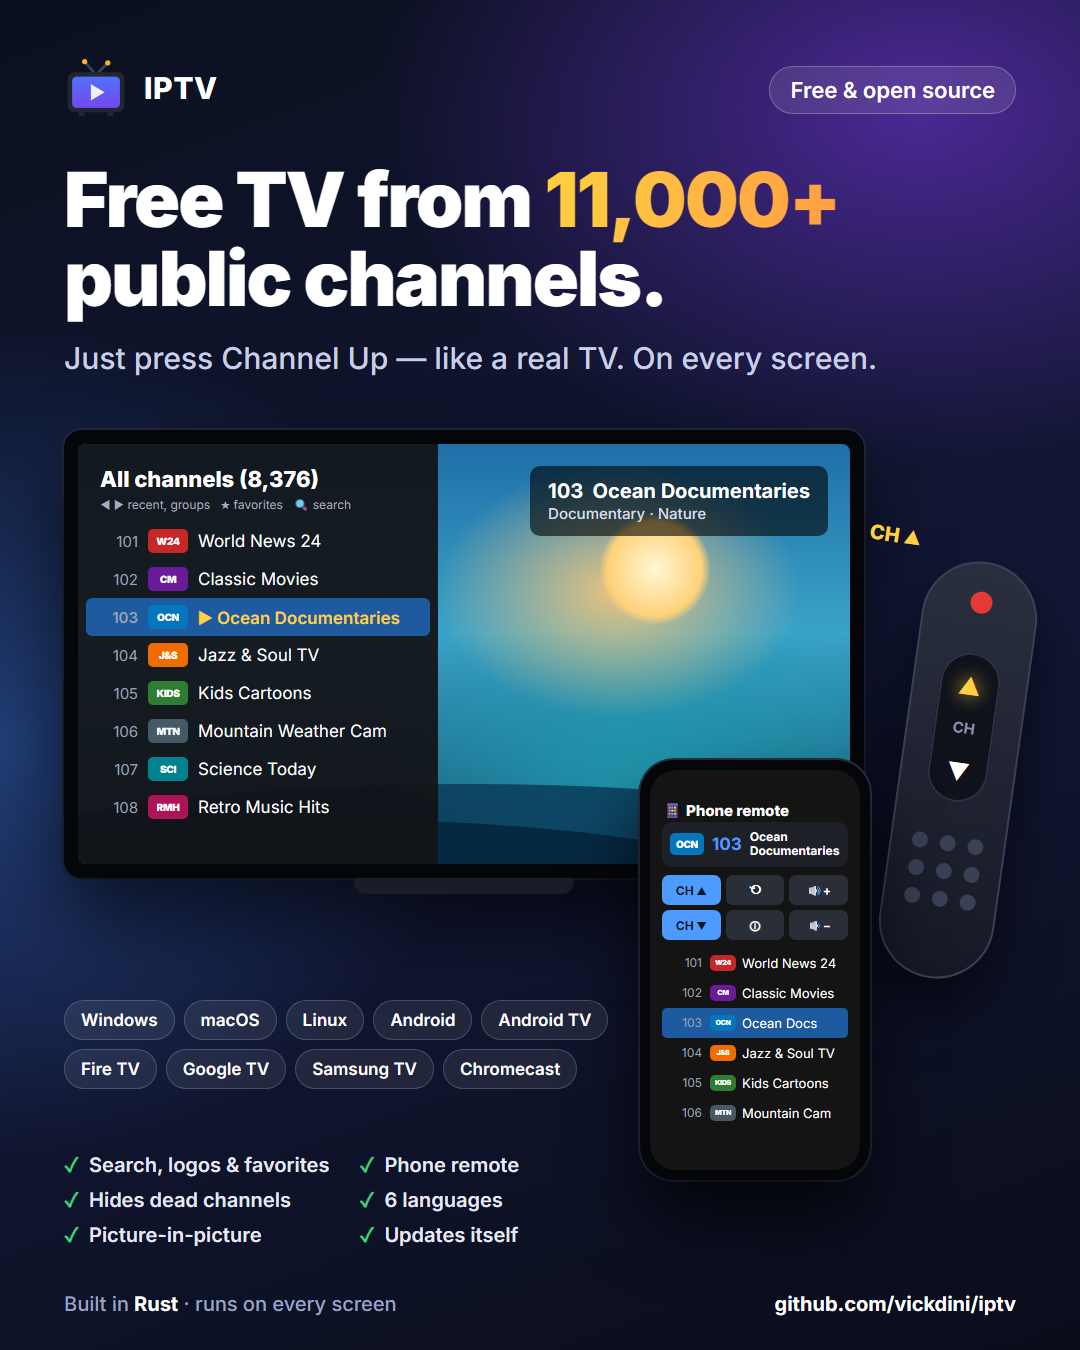
\includegraphics[width=0.52\textwidth]{../images/iptv-overview.png}\par
  \vfill
  {\large Windows \textbullet{} macOS \textbullet{} Linux \textbullet{} Android
   \textbullet{} Android TV \& Fire TV \textbullet{} Chromecast \textbullet{} Samsung TV\par}
  \vspace{0.5cm}
  {\color{dim} #2 \version{} \textbullet{} \url{https://github.com/vickdini/iptv}\par}
\end{titlepage}
\tableofcontents
\thispagestyle{fancy}}
:
%   \GuideLang   babel language (english, italian, spanish, french, ngerman, portuguese)
%   \GuideTitle  the guide's title, used on the cover, in headers and the PDF
%   \TipLabel    the word that starts a tip box ("Tip.")
% Build any of them with pdflatex, twice (for the table of contents).
\documentclass[11pt,a4paper]{article}

\usepackage[T1]{fontenc}
\usepackage[utf8]{inputenc}
% shorthands=off: no language-specific active characters (they would clash
% with tables and addresses); only hyphenation and "Contents" etc. change.
\usepackage[shorthands=off,\GuideLang]{babel}
\usepackage{lmodern}
\usepackage[scaled=0.92]{helvet}
\renewcommand{\familydefault}{\sfdefault}
\usepackage[margin=2.2cm,headheight=14pt]{geometry}
\usepackage{graphicx}
\usepackage[table]{xcolor}
\usepackage{booktabs}
\usepackage{tabularx}
\usepackage{xltabular}
\usepackage{enumitem}
\usepackage{titlesec}
\usepackage{fancyhdr}
\usepackage{pifont}
\usepackage{amssymb}
\usepackage[hidelinks]{hyperref}

\newcommand{\version}{0.12}
\definecolor{accent}{HTML}{1E6FD9}
\definecolor{dim}{HTML}{5F6673}
\definecolor{notebg}{HTML}{EEF4FC}
\definecolor{warnbg}{HTML}{FFF6E0}
\definecolor{tvred}{HTML}{D32F2F}
\definecolor{tvgreen}{HTML}{2E7D32}
\definecolor{tvyellow}{HTML}{C9A400}
\definecolor{tvblue}{HTML}{1565C0}

\hypersetup{pdftitle={IPTV -- \GuideTitle}, pdfauthor={IPTV project}}
\setlist{itemsep=2pt, topsep=4pt}
\setlength{\parindent}{0pt}
\setlength{\parskip}{6pt}
\renewcommand{\arraystretch}{1.25}

\titleformat{\section}{\Large\bfseries\color{accent}}{\thesection}{0.6em}{}
\titleformat{\subsection}{\large\bfseries}{\thesubsection}{0.6em}{}
\titlespacing*{\section}{0pt}{14pt}{6pt}
\titlespacing*{\subsection}{0pt}{10pt}{4pt}

\pagestyle{fancy}
\fancyhf{}
\fancyhead[L]{\small\color{dim}IPTV -- \GuideTitle}
\fancyhead[R]{\small\color{dim}github.com/vickdini/iptv}
\fancyfoot[C]{\small\color{dim}\thepage}
\renewcommand{\headrulewidth}{0.4pt}
\renewcommand{\sectionmark}[1]{\markboth{#1}{}}

% A key or button on a keyboard / remote.
\newcommand{\key}[1]{{\setlength{\fboxsep}{1.5pt}\fbox{\footnotesize\vphantom{Ay}#1}}}
% A coloured remote button.
\newcommand{\colorkey}[2]{\textcolor{#1}{\ding{108}}\,\textbf{#2}}
% Shaded boxes for tips and notes.
\newcommand{\tip}[1]{\par\noindent\colorbox{notebg}{\parbox{\dimexpr\linewidth-2\fboxsep}{\small\textbf{\TipLabel} #1}}\par}
\newcommand{\note}[1]{\par\noindent\colorbox{warnbg}{\parbox{\dimexpr\linewidth-2\fboxsep}{\small #1}}\par}
\newcommand{\menu}[1]{\textit{#1}}
\newcommand{\download}{\url{https://github.com/vickdini/iptv/releases/latest}}
% Key tables: \rowcolors{2}{gray!8}{white} then
% \begin{xltabular}{\linewidth}{@{}KX@{}} \keyshead{Key}{What it does} ... \bottomrule
\newcolumntype{K}{>{\raggedright\arraybackslash}p{5.4cm}}
\newcommand{\keyshead}[2]{\toprule \textbf{#1} & \textbf{#2} \\ \midrule}

% The cover: #1 subtitle, #2 "Version".
\newcommand{\cover}[2]{%
\begin{titlepage}
  \centering
  \vspace*{0.5cm}
  {\fontsize{40}{48}\selectfont\bfseries\color{accent} IPTV\par}
  \vspace{0.3cm}
  {\LARGE \GuideTitle\par}
  \vspace{0.3cm}
  {\large\color{dim} #1\par}
  \vspace{1cm}
  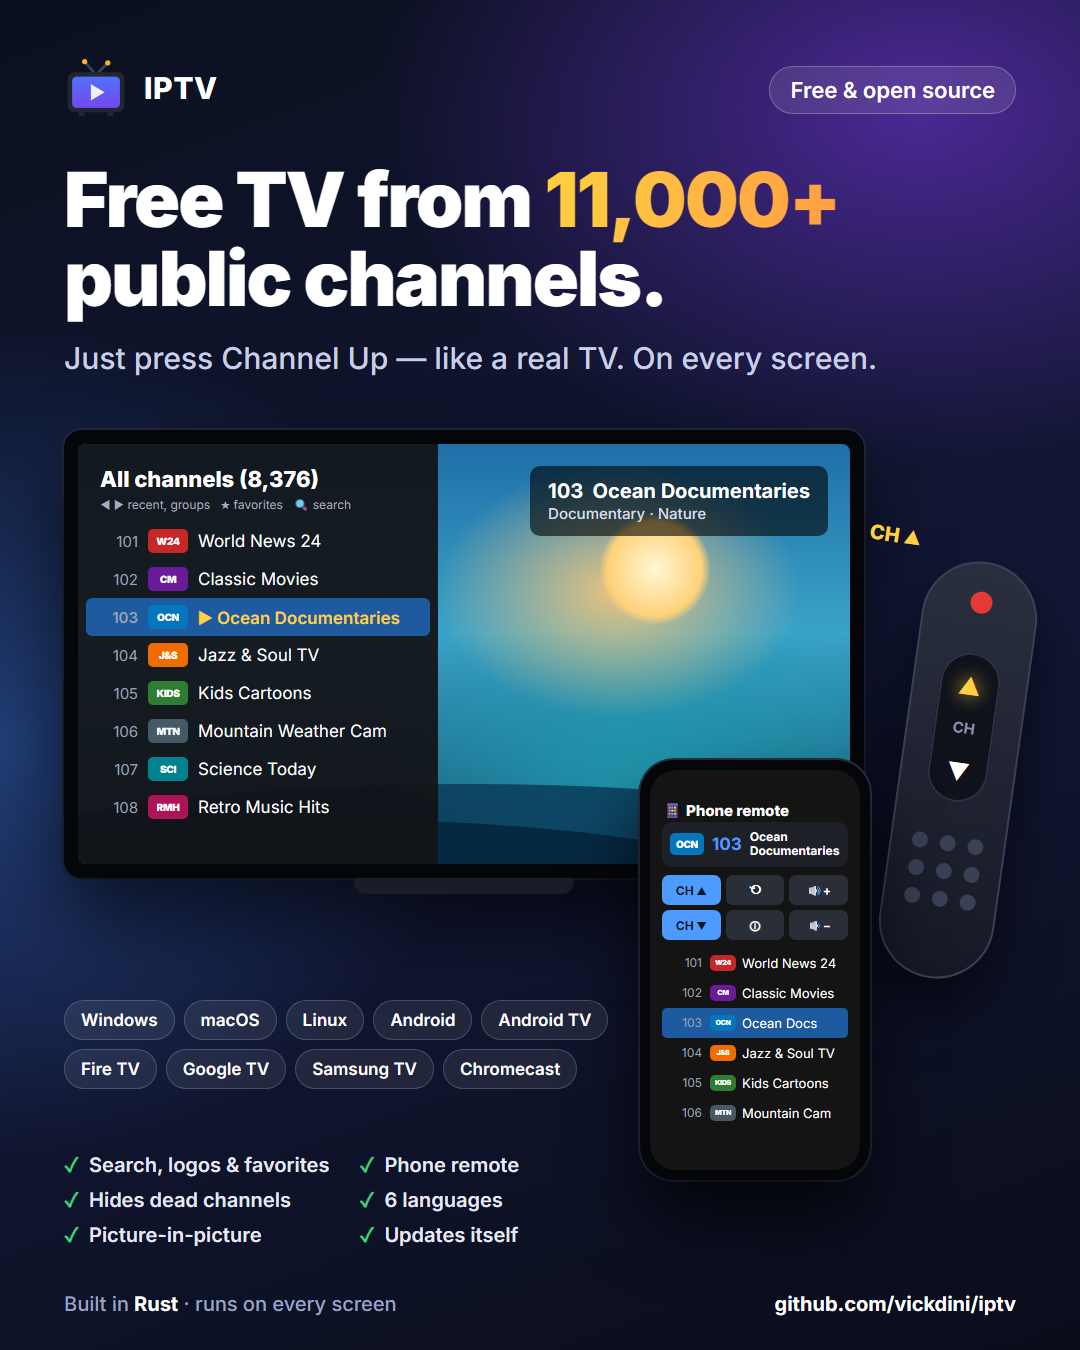
\includegraphics[width=0.52\textwidth]{../images/iptv-overview.png}\par
  \vfill
  {\large Windows \textbullet{} macOS \textbullet{} Linux \textbullet{} Android
   \textbullet{} Android TV \& Fire TV \textbullet{} Chromecast \textbullet{} Samsung TV\par}
  \vspace{0.5cm}
  {\color{dim} #2 \version{} \textbullet{} \url{https://github.com/vickdini/iptv}\par}
\end{titlepage}
\tableofcontents
\thispagestyle{fancy}}
:
%   \GuideLang   babel language (english, italian, spanish, french, ngerman, portuguese)
%   \GuideTitle  the guide's title, used on the cover, in headers and the PDF
%   \TipLabel    the word that starts a tip box ("Tip.")
% Build any of them with pdflatex, twice (for the table of contents).
\documentclass[11pt,a4paper]{article}

\usepackage[T1]{fontenc}
\usepackage[utf8]{inputenc}
% shorthands=off: no language-specific active characters (they would clash
% with tables and addresses); only hyphenation and "Contents" etc. change.
\usepackage[shorthands=off,\GuideLang]{babel}
\usepackage{lmodern}
\usepackage[scaled=0.92]{helvet}
\renewcommand{\familydefault}{\sfdefault}
\usepackage[margin=2.2cm,headheight=14pt]{geometry}
\usepackage{graphicx}
\usepackage[table]{xcolor}
\usepackage{booktabs}
\usepackage{tabularx}
\usepackage{xltabular}
\usepackage{enumitem}
\usepackage{titlesec}
\usepackage{fancyhdr}
\usepackage{pifont}
\usepackage{amssymb}
\usepackage[hidelinks]{hyperref}

\newcommand{\version}{0.12}
\definecolor{accent}{HTML}{1E6FD9}
\definecolor{dim}{HTML}{5F6673}
\definecolor{notebg}{HTML}{EEF4FC}
\definecolor{warnbg}{HTML}{FFF6E0}
\definecolor{tvred}{HTML}{D32F2F}
\definecolor{tvgreen}{HTML}{2E7D32}
\definecolor{tvyellow}{HTML}{C9A400}
\definecolor{tvblue}{HTML}{1565C0}

\hypersetup{pdftitle={IPTV -- \GuideTitle}, pdfauthor={IPTV project}}
\setlist{itemsep=2pt, topsep=4pt}
\setlength{\parindent}{0pt}
\setlength{\parskip}{6pt}
\renewcommand{\arraystretch}{1.25}

\titleformat{\section}{\Large\bfseries\color{accent}}{\thesection}{0.6em}{}
\titleformat{\subsection}{\large\bfseries}{\thesubsection}{0.6em}{}
\titlespacing*{\section}{0pt}{14pt}{6pt}
\titlespacing*{\subsection}{0pt}{10pt}{4pt}

\pagestyle{fancy}
\fancyhf{}
\fancyhead[L]{\small\color{dim}IPTV -- \GuideTitle}
\fancyhead[R]{\small\color{dim}github.com/vickdini/iptv}
\fancyfoot[C]{\small\color{dim}\thepage}
\renewcommand{\headrulewidth}{0.4pt}
\renewcommand{\sectionmark}[1]{\markboth{#1}{}}

% A key or button on a keyboard / remote.
\newcommand{\key}[1]{{\setlength{\fboxsep}{1.5pt}\fbox{\footnotesize\vphantom{Ay}#1}}}
% A coloured remote button.
\newcommand{\colorkey}[2]{\textcolor{#1}{\ding{108}}\,\textbf{#2}}
% Shaded boxes for tips and notes.
\newcommand{\tip}[1]{\par\noindent\colorbox{notebg}{\parbox{\dimexpr\linewidth-2\fboxsep}{\small\textbf{\TipLabel} #1}}\par}
\newcommand{\note}[1]{\par\noindent\colorbox{warnbg}{\parbox{\dimexpr\linewidth-2\fboxsep}{\small #1}}\par}
\newcommand{\menu}[1]{\textit{#1}}
\newcommand{\download}{\url{https://github.com/vickdini/iptv/releases/latest}}
% Key tables: \rowcolors{2}{gray!8}{white} then
% \begin{xltabular}{\linewidth}{@{}KX@{}} \keyshead{Key}{What it does} ... \bottomrule
\newcolumntype{K}{>{\raggedright\arraybackslash}p{5.4cm}}
\newcommand{\keyshead}[2]{\toprule \textbf{#1} & \textbf{#2} \\ \midrule}

% The cover: #1 subtitle, #2 "Version".
\newcommand{\cover}[2]{%
\begin{titlepage}
  \centering
  \vspace*{0.5cm}
  {\fontsize{40}{48}\selectfont\bfseries\color{accent} IPTV\par}
  \vspace{0.3cm}
  {\LARGE \GuideTitle\par}
  \vspace{0.3cm}
  {\large\color{dim} #1\par}
  \vspace{1cm}
  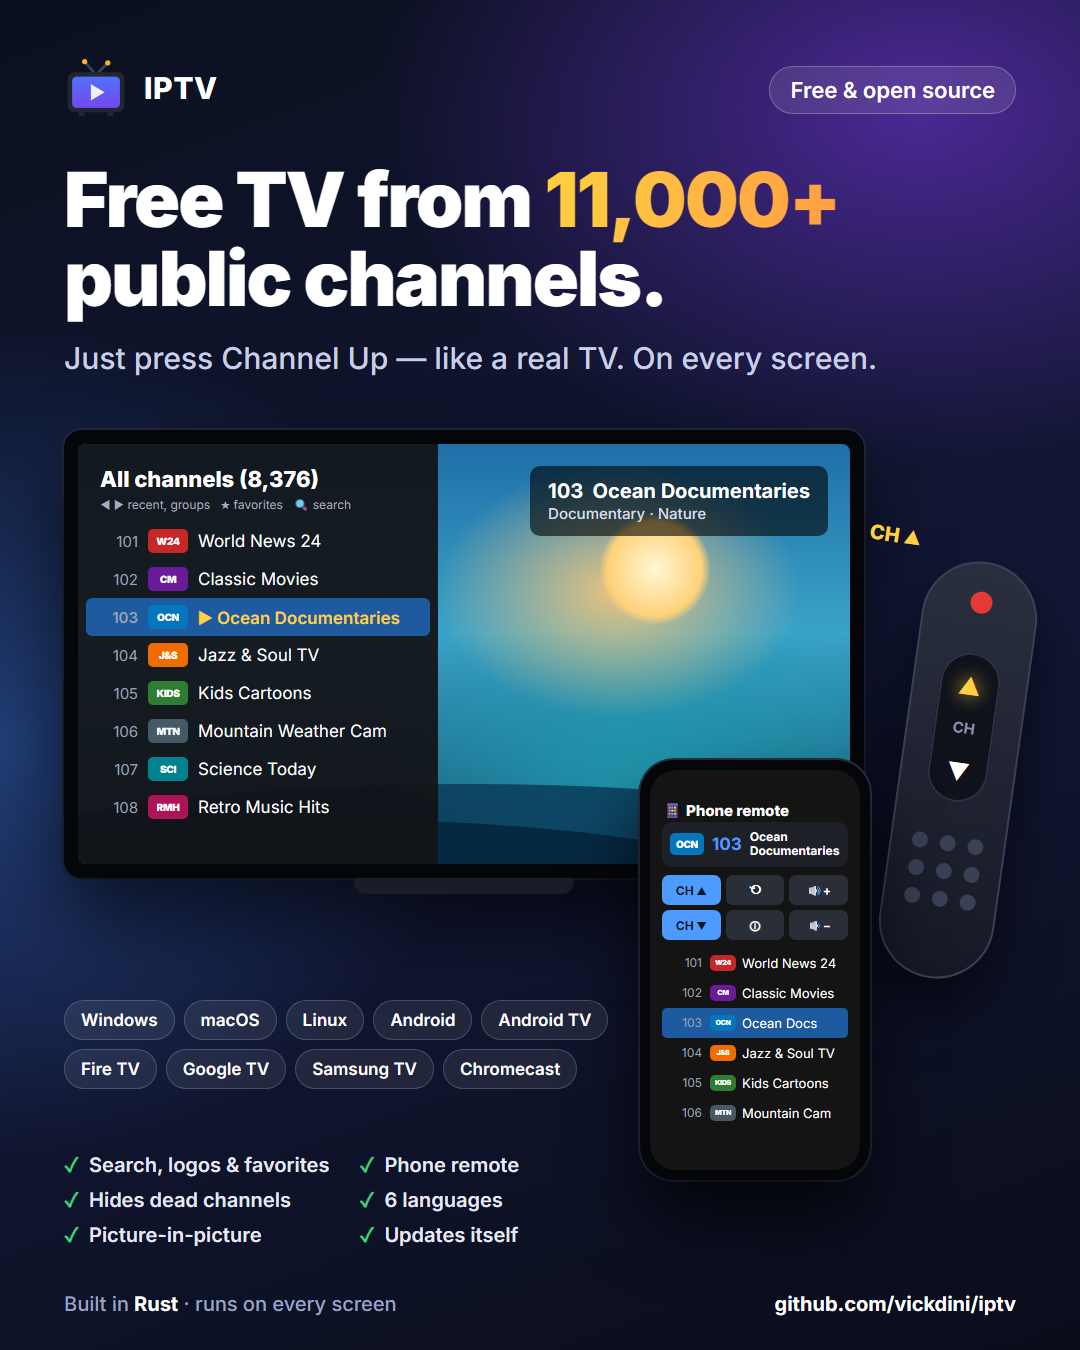
\includegraphics[width=0.52\textwidth]{../images/iptv-overview.png}\par
  \vfill
  {\large Windows \textbullet{} macOS \textbullet{} Linux \textbullet{} Android
   \textbullet{} Android TV \& Fire TV \textbullet{} Chromecast \textbullet{} Samsung TV\par}
  \vspace{0.5cm}
  {\color{dim} #2 \version{} \textbullet{} \url{https://github.com/vickdini/iptv}\par}
\end{titlepage}
\tableofcontents
\thispagestyle{fancy}}


\begin{document}
\cover{Mira canales de TV gratuitos y haz zapping como en un televisor}{Versión}

% ------------------------------------------------------------------ intro
\section{Qué es IPTV}

IPTV reproduce los canales de TV gratuitos y de acceso público que reúne el
proyecto \emph{iptv-org} (más de 10\,000) y te permite pasar de uno a otro
como en un televisor: subir y bajar de canal, números de canal, favoritos y
grupos como Noticias, Películas o Deportes.

\begin{itemize}
  \item \textbf{Siempre al día.} La lista de canales se actualiza cada vez
        que se abre IPTV, y la aplicación se actualiza sola cuando sale una
        versión nueva.
  \item \textbf{Solo canales que funcionan.} Los canales caídos se ocultan
        automáticamente, así el zapping nunca se queda en una pantalla negra.
  \item \textbf{Encuentra canales enseguida.} Busca por nombre, reconoce cada
        canal por su logotipo, vuelve a los canales vistos recientemente o
        muestra solo los países e idiomas que te interesan.
  \item \textbf{Tu idioma.} IPTV habla español, inglés, italiano, francés,
        alemán y portugués, y sigue el idioma de tu dispositivo. En los
        canales que lo emiten, elige el idioma del audio y activa los
        subtítulos.
  \item \textbf{Mando desde el móvil.} Controla la TV o el ordenador desde el
        navegador del móvil (sección~\ref{sec:remote}).
\end{itemize}

Cada descarga incluye todo lo necesario: no hay que instalar nada más. Todas
las descargas están en la página de versiones:

\begin{center}
  \download
\end{center}

\note{\textbf{Aviso.} IPTV no aloja ni ofrece ningún vídeo: solo carga una
lista pública publicada por el proyecto iptv-org. Mira solo lo que la ley de
tu país te permita ver.}

% ------------------------------------------------------------------ Windows
\section{Windows}
\label{sec:windows}

\subsection{Instalación}
\begin{enumerate}
  \item Descarga \texttt{IPTV-Setup-\textless versión\textgreater.exe} de la
        página de versiones y ábrelo.
  \item Si Windows muestra \menu{Windows protegió su PC}, haz clic en
        \menu{Más información} y después en \menu{Ejecutar de todas formas}.
  \item Sigue el instalador. No necesita permisos de administrador y añade
        un acceso directo en el menú Inicio (y un icono en el escritorio, si
        quieres).
\end{enumerate}
IPTV se abre maximizado y empieza a reproducir enseguida. Para quitarlo, usa
\menu{Configuración \textrightarrow{} Aplicaciones}.

\subsection{Teclas}
\label{sec:keys}
Estas teclas funcionan en todos los ordenadores: Windows, macOS y Linux.

\rowcolors{2}{gray!8}{white}
\begin{xltabular}{\linewidth}{@{}KX@{}}
\keyshead{Tecla}{Qué hace}
\key{$\uparrow$} \key{$\downarrow$}, \key{RePág} \key{AvPág}, rueda del ratón & canal siguiente / anterior \\
\key{0}--\key{9}, luego espera o \key{Intro} & ir a un número de canal \\
\key{Retroceso} & volver al canal anterior \\
\key{$\leftarrow$} \key{$\rightarrow$}, \key{m} & bajar / subir el volumen, silencio \\
\key{l}, \key{Tab} o clic derecho & abrir / cerrar la lista de canales \\
\key{/} o \key{Ctrl}+\key{F} & buscar canales por nombre \\
\key{c} & elegir países e idiomas \\
\key{g} / \key{G} & vistos recientemente y luego los grupos (Noticias, Películas\ldots) \\
\key{s} / \key{S} & marcar o quitar un favorito / zapping solo entre favoritos \\
\key{a} / \key{t} & siguiente idioma del audio / siguientes subtítulos (y desactivados) \\
\key{r} & mando desde el móvil: mostrar el código QR \\
\key{E} / \key{I} & exportar / importar favoritos (carpeta Descargas) \\
\key{i} & información del canal \\
\key{f}, doble clic & pantalla completa (\key{Esc} para salir) \\
\key{p} & imagen pequeña: un segundo canal, pequeño, en la esquina inferior derecha \\
\key{[} / \key{]} & canal anterior / siguiente de la imagen pequeña \\
\key{x}, clic en la imagen pequeña & intercambiar los dos canales \\
\key{Espacio} & pausa \\
\key{h}, \key{?} o \key{F1} & ayuda en pantalla \\
\key{q} & salir \\
\bottomrule
\end{xltabular}

\subsection{La lista de canales}
Pulsa \key{l} para abrir a la izquierda una lista desplazable de canales, con
sus logotipos; el vídeo sigue al lado. Desplázate con la rueda del ratón y
haz clic en un canal para verlo. Empieza a escribir (o pulsa \key{/}) para
buscar: las tildes y las mayúsculas dan igual. \key{Esc} cierra la lista.
Pulsa \key{g} para ver los canales vistos recientemente, del más reciente al
más antiguo.

\subsection{Países e idiomas}
Pulsa \key{c}, escribe para buscar un país o un idioma y pulsa \key{Intro}
para marcarlo; \key{Tab} cambia entre las dos listas. A partir de ahí IPTV
solo muestra los canales de los países marcados o en los idiomas marcados,
hasta que borres la selección (\key{Supr}, o la fila \emph{Quitar todos los
filtros}).

\subsection{Idioma del audio y subtítulos}
Cuando un canal ofrece más de un idioma de audio o subtítulos, una nota en la
parte inferior de la pantalla lo indica. Pulsa \key{a} para el siguiente
idioma del audio y \key{t} para los siguientes subtítulos (y al final
\emph{desactivados}). IPTV recuerda el idioma y lo usa en todos los demás
canales que lo ofrecen.

\subsection{Idioma y actualizaciones}
IPTV usa el idioma del sistema. Cada vez que se abre comprueba si hay una
versión nueva; si la hay, la instala sin preguntar y se reinicia solo al cabo
de unos segundos.

% ------------------------------------------------------------------ macOS
\section{macOS}

\subsection{Instalación}
\begin{enumerate}
  \item Comprueba qué chip tiene tu Mac: \menu{menú Apple \textrightarrow{}
        Acerca de este Mac}.
  \item Descarga la imagen de disco correspondiente de la página de
        versiones:
  \begin{itemize}
    \item Apple silicon (M1, M2, M3, M4\ldots):
          \texttt{IPTV-\textless versión\textgreater-macOS-arm64.dmg}
    \item Intel: \texttt{IPTV-\textless versión\textgreater-macOS-x86\_64.dmg}
  \end{itemize}
  \item Ábrela y arrastra \textbf{IPTV} a \textbf{Aplicaciones}.
\end{enumerate}

\subsection{Primer arranque}
IPTV no está notarizado por Apple, así que la primera vez macOS se niega a
abrirlo. Solo hace falta una vez:
\begin{enumerate}
  \item Abre IPTV desde Aplicaciones. Cuando macOS diga que no se puede abrir,
        haz clic en \menu{OK}.
  \item Abre \menu{Ajustes del Sistema \textrightarrow{} Privacidad y
        seguridad}, baja hasta \menu{Se ha bloqueado «IPTV»\ldots} y haz clic
        en \menu{Abrir igualmente}; después confirma.
\end{enumerate}

\subsection{Uso}
IPTV usa las mismas teclas que en Windows (sección~\ref{sec:keys}). En el
Dock aparece como \textbf{IPTV} mientras reproduce un canal.

\tip{Guarda IPTV en la carpeta Aplicaciones: si se abre desde la imagen de
disco o desde Descargas, macOS lo ejecuta desde una copia de solo lectura y no
puede actualizarse.}

% ------------------------------------------------------------------ Linux
\section{Linux}

\subsection{Instalación}
Descarga \texttt{IPTV-\textless versión\textgreater-x86\_64.AppImage} de la
página de versiones. Es un único archivo que lo incluye todo. Hazlo
ejecutable y ábrelo:
\begin{center}
\begin{minipage}{0.8\linewidth}
\small\ttfamily chmod +x IPTV-*-x86\_64.AppImage\\
./IPTV-*-x86\_64.AppImage
\end{minipage}
\end{center}
También puedes, en un gestor de archivos, abrir \menu{Propiedades
\textrightarrow{} Permisos}, marcar \menu{Permitir ejecutar el archivo como
un programa} y hacer doble clic en él.

Funciona en PC de 64 bits con un Linux de 2022 o posterior (Ubuntu 22.04,
Debian 12, Fedora 36, Linux Mint 21 y versiones más recientes).

\tip{Herramientas como \emph{Gear Lever} o \emph{AppImageLauncher} añaden
IPTV al menú de aplicaciones. Si el AppImage dice que falta FUSE, ábrelo con
\texttt{-{}-appimage-extract-and-run}.}

\subsection{Uso}
IPTV usa las mismas teclas que en Windows (sección~\ref{sec:keys}). Se
actualiza sustituyendo el archivo AppImage, así que guárdalo en una carpeta en
la que puedas escribir (por ejemplo, tu carpeta personal).

% ------------------------------------------------------------------ Android
\section{Móviles y tabletas Android}

\subsection{Instalación}
\begin{enumerate}
  \item En el móvil, descarga \texttt{IPTV-\textless versión\textgreater.apk}
        de la página de versiones y ábrelo.
  \item Android pide una vez permiso para instalar aplicaciones desde el
        navegador o el gestor de archivos: permítelo y toca \menu{Instalar}.
  \item IPTV no está en Google Play, así que Play Protect puede avisar de un
        desarrollador desconocido: elige \menu{Instalar de todas formas}.
\end{enumerate}
También puedes instalarlo con \emph{Obtainium}, que mantiene las
aplicaciones actualizadas directamente desde su página de versiones.

\subsection{Gestos}
\rowcolors{2}{gray!8}{white}
\begin{xltabular}{\linewidth}{@{}KX@{}}
\keyshead{Gesto}{Qué hace}
deslizar hacia arriba / abajo & canal siguiente / anterior \\
tocar & abrir / cerrar la lista de canales \\
doble toque & volver al canal anterior \\
mantener pulsado & información del canal \\
\bottomrule
\end{xltabular}

\subsection{Dos canales a la vez}
Pon el móvil o la tableta en vertical y la pantalla se divide en dos, un
canal encima del otro. Toca una mitad para oírla: un borde azul fino la
señala, y la lista de canales y el mando desde el móvil actúan sobre ella.
Desliza hacia arriba o abajo sobre una mitad para cambiar su canal. Vuelve a
poner el dispositivo en horizontal para ver un solo canal.

\subsection{Imagen en imagen}
Sal de la aplicación mientras ves algo (botón de inicio, o desliza hacia
arriba desde abajo): el canal sigue en una ventana pequeña sobre las demás
aplicaciones, con botones para cambiar de canal. Toca la ventana para volver a
IPTV, o arrástrala fuera para cerrarla. Necesita Android 8 o posterior.

Con la pantalla apagada o el móvil bloqueado, el canal sigue sonando: la
pantalla de bloqueo lo muestra, con botones para cambiar de canal o
detenerlo.

\subsection{La lista de canales}
Toca la pantalla para abrirla. Toca un canal para verlo, mantenlo pulsado
para añadirlo a favoritos o quitarlo. Los botones de arriba:
\begin{itemize}
  \item Casilla de \textbf{búsqueda}: escribe parte del nombre de un canal.
  \item Flechas $\blacktriangleleft$\,$\blacktriangleright$: grupo anterior /
        siguiente.
  \item \textbf{Reloj}: los canales vistos recientemente.
  \item $\bigstar$: solo favoritos. Mantenlo pulsado para guardar tus
        favoritos en un archivo o añadirlos desde uno.
  \item \textbf{Globo}: elegir países e idiomas.
  \item \textbf{Subtítulos} (solo en canales que ofrecen opciones): idioma
        del audio y subtítulos.
  \item \textbf{Mando desde el móvil}: controla IPTV desde otro móvil
        (sección~\ref{sec:remote}).
  \item \textbf{Enviar}: reproducir en un Chromecast
        (sección~\ref{sec:chromecast}).
  \item \textbf{Salir}: cierra IPTV (y deja de enviar).
\end{itemize}

\subsection{Idioma y actualizaciones}
IPTV usa el idioma del móvil. Al abrirse comprueba si hay una versión nueva.
La primera vez, Android pide permitir que IPTV instale aplicaciones; después,
las actualizaciones se instalan con una confirmación como mucho.

% ------------------------------------------------------------------ Android TV
\section{Android TV, Google TV y Fire TV}

La misma aplicación funciona en dispositivos de TV y se maneja con el mando.
Las tiendas de TV no la ofrecen, así que se instala una vez con la aplicación
gratuita \emph{Downloader}:

\begin{itemize}
  \item \textbf{Fire TV / Fire TV Stick:} instala \emph{Downloader} desde la
        tienda de Amazon. Después abre \menu{Configuración \textrightarrow{} Mi
        Fire TV \textrightarrow{} Opciones para desarrolladores
        \textrightarrow{} Instalar aplicaciones desconocidas} y activa
        Downloader.
  \item \textbf{Google TV, Chromecast con Google TV, Android TV:} instala
        \emph{Downloader} desde Play Store y permítelo en
        \menu{Ajustes \textrightarrow{} Aplicaciones \textrightarrow{}
        Seguridad y restricciones \textrightarrow{} Fuentes desconocidas}.
\end{itemize}
En Downloader, escribe
\begin{center}
  \download
\end{center}
y después descarga \texttt{IPTV-\textless versión\textgreater.apk} e
instálalo. IPTV aparecerá entre las aplicaciones de la TV.

\subsection{Mando a distancia}
\rowcolors{2}{gray!8}{white}
\begin{xltabular}{\linewidth}{@{}KX@{}}
\keyshead{Botón}{Qué hace}
Arriba / Abajo, Canal +/$-$, Avance / Retroceso rápido & canal siguiente / anterior \\
OK, Reproducir/Pausa, Menú & abrir / cerrar la lista de canales \\
Izquierda / Derecha & vistos recientemente y luego los grupos \\
0--9 (si el mando los tiene) & ir a un número de canal \\
Atrás & cerrar la lista \\
Info & información del canal \\
Teclas Audio / CC (si las hay) & siguiente idioma del audio / subtítulos \\
\bottomrule
\end{xltabular}

En la lista de canales, pulsa Arriba sobre el primer canal para llegar a la
casilla de búsqueda. Los botones de arriba de la lista eligen países e
idiomas, audio y subtítulos, y abren el mando desde el móvil.

\tip{La mayoría de estos mandos no tiene teclas numéricas: el mando desde el
móvil (sección~\ref{sec:remote}) es la forma más rápida de elegir un canal.}

% ------------------------------------------------------------------ Chromecast
\section{Chromecast}
\label{sec:chromecast}

Los Chromecast antiguos (el dispositivo sencillo sin mando) no pueden
instalar aplicaciones. Envía a ellos desde la aplicación de Android:
\begin{enumerate}
  \item Comprueba que el móvil y el Chromecast estén en la misma Wi-Fi.
  \item Abre la lista de canales en IPTV, toca el botón \textbf{Enviar} y
        elige tu Chromecast.
  \item Haz zapping en el móvil como siempre: la TV le sigue.
\end{enumerate}
Algunos canales no se pueden enviar porque sus servidores no lo permiten;
IPTV los salta automáticamente.

% ------------------------------------------------------------------ Samsung
\section{Smart TV Samsung}

IPTV funciona en los televisores Samsung de 2019 en adelante. Samsung solo
permite instalar aplicaciones que no están en su tienda desde un ordenador,
con la TV en \emph{modo desarrollador}. La configuración se hace una sola vez,
desde un PC con Windows en la misma Wi-Fi que la TV.

\subsection{Instalación}
\begin{enumerate}
  \item En el PC, instala desde \url{https://developer.tizen.org} las
        herramientas de línea de comandos de \emph{Tizen Studio}. En su
        Package Manager, instala \emph{Samsung Certificate Extension} y
        \emph{TV Extensions Tools} (pestaña \menu{Extension SDK}).
  \item En la TV, abre \menu{Aplicaciones} y escribe
        \key{1}\key{2}\key{3}\key{4}\key{5} con el mando. Activa el
        \menu{modo desarrollador}, introduce la dirección IP del PC y reinicia
        la TV.
  \item Descarga \texttt{IPTV-Samsung-TV-\textless versión\textgreater.zip}
        de la página de versiones y descomprímelo.
  \item Busca la dirección IP de la TV (\menu{Configuración \textrightarrow{}
        General \textrightarrow{} Red \textrightarrow{} Estado de red}) y
        ejecuta, en la carpeta descomprimida:
\begin{center}
\begin{minipage}{0.92\linewidth}
\small\ttfamily powershell -ExecutionPolicy Bypass -File install-on-tv.ps1 -TvIp 192.168.1.4
\end{minipage}
\end{center}
        La primera vez explica cómo crear el certificado gratuito de Samsung
        (con una cuenta Samsung). Ejecútalo de nuevo después: instala IPTV,
        que aparecerá entre las aplicaciones de la TV.
\end{enumerate}
A partir de ahí IPTV se actualiza solo: no hace falta repetir la
configuración para las versiones nuevas. Usa el idioma de la TV.

\subsection{Mando a distancia}
\rowcolors{2}{gray!8}{white}
\begin{xltabular}{\linewidth}{@{}KX@{}}
\keyshead{Botón}{Qué hace}
Arriba / Abajo, CH + / CH $-$ & canal siguiente / anterior \\
0--9 & ir a un número de canal \\
OK & lista de canales (en la lista: ver el canal seleccionado) \\
Izquierda / Derecha & vistos recientemente y luego los grupos \\
PRE-CH & volver al canal anterior \\
INFO & información del canal \\
\colorkey{tvred}{Rojo} & añadir o quitar un favorito \\
\colorkey{tvgreen}{Verde} & solo favoritos \\
\colorkey{tvyellow}{Amarillo} & menú de idioma del audio y subtítulos \\
\colorkey{tvyellow}{Amarillo} en la lista & elegir países e idiomas \\
\colorkey{tvblue}{Azul} & buscar canales por nombre \\
Atrás & cerrar la lista o salir de IPTV \\
\bottomrule
\end{xltabular}

\note{El mando desde el móvil (sección~\ref{sec:remote}) aún no está
disponible en los televisores Samsung. La aplicación gratuita
\emph{SmartThings} sirve como mando desde el móvil para los botones básicos.}

% ------------------------------------------------------------------ remote
\section{Mando desde el móvil}
\label{sec:remote}

Controla IPTV desde tu móvil, Android o iPhone, sin instalar nada. Puedes
recorrer y buscar todos los canales y tocar uno para verlo; el mando también
tiene favoritos, canales vistos recientemente, canal arriba / abajo, volumen,
idioma del audio y subtítulos. Funciona con IPTV en un ordenador y en Android
TV, Google TV y Fire TV, y habla el idioma de tu móvil.

\begin{enumerate}
  \item En un ordenador pulsa \key{r}. En Android TV, Google TV o Fire TV,
        abre la lista de canales y elige el botón \textbf{mando desde el
        móvil}. Aparece un código QR.
  \item Escanéalo con la cámara del móvil. El móvil tiene que estar en la
        misma Wi-Fi. Sin cámara, abre en el navegador del móvil la dirección
        que aparece en pantalla y escribe el PIN.
  \item El mando se abre en el navegador del móvil. Añádelo a la pantalla de
        inicio o a marcadores: desde entonces se conecta solo siempre que
        IPTV esté abierto.
\end{enumerate}

Para llevar tus favoritos a otra TV u otro ordenador, usa \textbf{Guardar en
el móvil} al final de la página del mando y después \textbf{Añadir desde un
archivo} en el mando del otro dispositivo. Los favoritos se añaden, nunca se
quitan. En un ordenador también puedes pulsar \key{E} (guardar en la carpeta
Descargas) e \key{I} (añadir desde ahí); en móviles y tabletas Android,
mantén pulsado el botón $\bigstar$.

\note{La primera vez, Windows (y macOS, si tiene el cortafuegos activado)
pregunta si IPTV puede usar la red: permítelo en las redes
\textbf{privadas}; si no, los móviles no podrán conectarse. Solo los móviles
que conocen el PIN pueden controlar IPTV.}

% ------------------------------------------------------------------ help
\section{Solución de problemas}

\begin{description}[style=nextline, leftmargin=0pt, itemsep=6pt]
  \item[Un canal no se reproduce.] Muchos canales gratuitos dejan de emitir o
        solo funcionan en algunos países. IPTV los oculta y pasa al siguiente
        solo; simplemente cambia de canal.
  \item[La lista parece más corta que antes.] Comprueba si hay países o
        idiomas elegidos (\key{c} en un ordenador, el botón del globo en
        Android, \colorkey{tvyellow}{Amarillo} en la lista en los televisores
        Samsung) y quítalos.
  \item[El mando desde el móvil no se conecta.] Comprueba que el móvil esté
        en la misma Wi-Fi (no en datos móviles) y que el cortafuegos del
        ordenador permita IPTV en las redes privadas.
  \item[Aparecen subtítulos en la lista pero no se ve nada.] Algunos canales
        anuncian subtítulos que en realidad no envían. IPTV funciona bien.
  \item[IPTV está en otro idioma.] Sigue el idioma del dispositivo (en un
        ordenador, el del sistema). Los nombres de canales, grupos y países
        vienen de la lista y siempre están en inglés.
  \item[¿Otra cosa?] Avísanos en
        \url{https://github.com/vickdini/iptv/issues}.
\end{description}

\vfill
{\small\color{dim} IPTV es software libre con licencia GNU General Public
License, versión 3 o posterior. Su código fuente está en
\url{https://github.com/vickdini/iptv}.\par}

\end{document}
